\vspace{-2mm}
\section{Parallelizing DeltaNet Across the Sequence Dimension}
% \vspace{-2mm}

% In the same spirit as the chunkwise form of linear attention, we derive a chunkwise form for DeltaNet that enables hardware-efficient training through parallelizing across the sequence dimension. 

\vspace{-2mm}
\subsection{A Memory-efficient Reparameterization}
\label{ssec:wy}
\vspace{-2mm}

We first observe that  $\rmS_t$ admits a purely additive representation of the form $\rmS_t = \sum_{i=1}^t \vu_i \vk_i^\intercal$ for $\vu_i, \vk_i \in \mathbb{R}^{d}$, since we can simply set $\vu_i = \vv_i^{\text{new}} - \vv_i^{\text{old}} = \beta_i(\vv_i - \vv_i^\text{old})$.
Recall from \S\ref{ssec:la} that simple linear attention has the form $\rmS_t = \sum_{i=1}^t \vv_i\vk_i^\intercal$. Thus, DeltaNet simply replaces the value vector $\vv_i$ in linear attention with the ``pseudo'' value vector $\vu_i$.
Once the $\vu_i$'s have been constructed, the rest of computation can proceed  as in ordinary linear attention, i.e., $\rmO = \left(\rmQ \rmK^\intercal \odot \rmM \ \right ) \rmU$ where $\rmU \in \mathbb{R}^{L \times d}$ is the row-wise concatenation of the $\vu_i$ vectors.

However, computing $\vu_t$ na\"{i}vely requires explicitly materializing  $\rmS_{t-1}$ to compute $\vv_t^{\text{old}}$, which would require $\mathcal{O}(d^2)$ memory. We now show that we can obtain the $\vu_t$'s \emph{without} explicitly materializing $\rmS_{t-1}$  in $\mathcal{O}(d)$ memory. 
Our simple proof (by induction) relies  on an application of the WY representation for products of Householder matrices  \cite{bischof_wy_1985}. The base case is clear since  we have $\rmS_1 = \beta_1 \vv_1 \vk_1^\intercal$, so $\vu_1 = \beta_1\vv_1$.
For the inductive step, we first observe that the DeltaNet update is given by,
\begin{align*}
    \rmS_t &= \rmS_{t-1} -\vv_t^{\text{old}}\vk_t^\intercal+\vv_t^{\text{new} }\vk_t^\intercal\nonumber  =  \rmS_{t-1} - \beta_t \left(\rmS_{t-1} \vk_t\right)\vk_t^\intercal + \beta_t \vv_t \vk_t^\intercal  = \rmS_{t-1} (\rmI - \beta_t \vk_t \vk_t^\intercal) + \beta_t \vv_t  \vk_t^\intercal,
\end{align*}
which can be seen as applying a generalized Householder transformation (i.e., matmul with an identity plus rank-one matrix) to the previous state. The inductive step is then given by,
\begin{align}
    \rmS_t & = \rmS_{t-1} (\rmI - \beta_t \vk_t\vk_t^\intercal) + \beta_t \vv_t  \vk_t^\intercal 
    = \sum_{i=1}^{t-1} \vu_{i}\vk_{i}^\intercal + \underbrace{\beta_t \left(\vv_t - \sum_{i=1}^{t-1} \vu_i \left(\vk_i^{\intercal} \vk_t \right)  \right)}_{\text{defined as } \vu_t} \vk_t^{\intercal} = \sum_{i=1}^{t} \vu_i \vk_i^\intercal
\label{eq:delta_KU}
\end{align}
Note that $\vu_t$ does not require materializing  any of the hidden states and requires $\mathcal{O}(d)$ memory to compute, thus completing the proof. While we have  avoided materializing  $\rmS_{t}$'s,  computing  $\vu_t$'s for all $L$ (that is, $\rmU$) takes $\mathcal{O}(L^2d)$ and moreover cannot be fully parallelized, unlike in linear attention where we can calculate all the value vectors $\rmV$ in parallel in $\mathcal{O}(1)$ steps. We now show that the above trick still enables an efficient chunkwise parallel form for  DeltaNet.

% , which similarly exploits the above representation for  products of Householder matrices.

\vspace{-2mm}
\subsection{Chunkwise Parallel Form for DeltaNet}
\label{sec:chunk_deltanet}
\vspace{-2mm}
To derive the chunkwise parallel form, we first unroll the recurrence, 
\begin{align}
  % \rmH_1^t= 
  \rmS_t 
   = \rmS_{t-1} (\rmI - \beta_t \vk_t \vk_t^\intercal) + \beta_t \vv_t  \vk_t^\intercal 
  = \sum_{i=1}^t  \beta_i (\vv_i \vk_i^\intercal) \left( \prod_{j=i+1}^t  (\rmI - \beta_j \vk_j \vk_j^\intercal) \right). 
\label{eq:unroll}
\end{align}
We then define the following variables: 
$\rmP_{i}^{j} =  \prod_{t=i}^j  (\rmI - \beta_t \vk_t \vk_t^\intercal)  \in \R^{d \times d}$,  $\rmH_{i}^{j} = \sum_{t=i}^j  \beta_t (\vv_t \vk_t^\intercal) \rmP_{t+1}^{j} \in \R^{d \times d}$, where we let $\rmP_{i}^j = \rmI$ whenever $i > j$. Intuitively, $\rmP_{i}^{j}$ is the ``decay factor'' to be applied to $\rmS_{i}$ for obtaining $\rmS_{j}$, and  $\rmH_{i}^{j}$ represents the   contributions to $\rmS_j$ starting from token $i$. (Hence $\rmS_{t} = \rmH_{1}^t$). The chunkwise recurrence  can then  be written as,
\begin{align}
    \rmS_{[t]}^{r} = \rmS_{[t]}^0 \rmP_{[t]}^{r} + \rmH_{[t]}^{r} 
     \label{eq:delta_chunk}
\end{align}
 where we define the chunkwise variables  $\rmS_{[t]}^i = \rmS_{tC + i}$,  $ \rmP_{[t]}^{r} = \rmP_{tC+1}^{tC+r}$, $\rmH_{[t]}^{r} =\rmH_{tC+1}^{tC+r}$.  Here we have $\frac{L}{C}$ chunks of size $C$. 
%
The trick is to now efficiently represent the $\rmP_{[t]}^r, \rmH_{[t]}^r \in \R^{d \times d}$ matrices using a similar approach described in \S\ref{ssec:wy}, so that these matrices can be stored in $\mathcal{O}(d)$ memory,
\begin{align}
    \rmP_{[t]}^{r} &= \rmI - \sum_{i=1}^{r}\vw_{[t]}^i\vk_{[t]}^{i\intercal}  ,\qquad \rmH_{[t]}^{r} = \sum_{i=1}^{r} \vu_{[t]}^i \vk_{[t]}^{i\intercal} \hspace{4mm} \in \R^{d \times d} \label{eq:wy-ph} \\
    \vw_{[t]}^r &= \beta_{[t]}^r \left(\vk_{[t]}^r -  \sum_{i=1}^{r-1} \vw_{[t]}^i (\vk_{[t]}^{i\intercal}\vk_{[t]}^r)  \right), \hspace{3mm}
    \vu_{[t]}^r = \beta_{[t]}^r \left(\vv_{[t]}^r -  \sum_{i=1}^{r-1} \vu_{[t]}^i (\vk_{[t]}^{i\intercal}\vk_{[t]}^r)  \right) \hspace{3mm} \in \R^{d} 
    \label{eq:wy-u}
\end{align}
The derivations for the above can be found in the appendix. Subsequently, based on Eq.~\ref{eq:delta_chunk}, we can obtain the chunk-level recurrence for hidden states and outputs as,
\begin{align*}
    \rmS_{[t]}^r &= \rmS_{[t]}^0 - \left(\rmS_{[t]}^0 \sum_{i=1}^{r}\vw_{[t]}^i \vk_{[t]}^{i\intercal} \right)+  \sum_{i=1}^{r} \vu_{[t]}^i \vk_{[t]}^{i\intercal} = \rmS_{[t]}^0 + \sum_{i=1}^{r} \left( \vu_{[t]}^i - \rmS_{[t]}^0 \vw_{[t]}^i \right) \vk_{[t]}^{i\intercal},  \\
\vo_{[t]}^r &= \rmS_{[t]}^r \vq_{[t]}^r   
            = \rmS_{[t]}^0 \vq_{[t]}^r + \sum_{i=1}^{r} \left( \vu_{[t]}^i - \rmS_{[t]}^0 \vw_{[t]}^i\right) \left(\vk_{[t]}^{i\intercal}\vq_ {[t]}^i\right).
\end{align*}
Letting  $\rmS_{[t]}=\rmS_{[t]}^0$, the above can be simplified to matrix notations similarly to Eq.\ref{eq:linear_attn_h}-\ref{eq:linear_attn_o},
\vspace{-3mm}
\begin{align}
\rmS_{[t+1]} &= \rmS_{[t]} + \left(\rmU_{[t]} -  \rmW_{[t]}\rmS_{[t]}^{\intercal}\right)^\intercal \rmK_{[t]},
\label{eq:delta_chunk_h} \\
    \rmO_{[t]} &= \rmQ_{[t]} \rmS_{[t]}^\intercal + (\rmQ_{[t]} \rmK_{[t]}^{\intercal} \odot \rmM) \left(\rmU_{[t]} - \rmW_{[t]} \rmS_{[t]}^\intercal\right)  \label{eq:delta_chunk_o}
\end{align}
where $\square_{[t]} = \square_{[t]}^{1:C} \in \mathbb{R}^{C\times d}$ for $\square \in \{\rmQ, \rmK, \rmV, \rmO, \rmU, \rmW \}$ defines the chunkwise matrices that are formed from stacking the $\vq_t, \vk_t, \vv_t, \vo_t, \vu_t, \vw_t$ vectors.

% \paragraph{UT transform for reducing non-matmul FLOPs.} 
\vspace{-2mm}
\paragraph{Practical considerations.} 
In the above, Eq. \ref{eq:wy-u} is fully recurrent and thus
cannot use tensor cores written as is.
 % The computations needed for constructing the chunkwise matrices $\rmU_{[t]}$'s and $\rmW_{[t]}$'s are strictly 
 % takes $\mathcal{O}(Ld)$ work but can  be parallelized across chunks, reducing the number of sequential steps from $L$ to $C$.
To solve this, we further leverage the \emph{UT transform} \cite{Joffrain2006AccumulatingHT, TomsDominguez2018FastBO} (see \S\ref{appendix:ut_transform} for derivations): 
 % We further leverage the compact UT transform 
\begin{align}
   \rmT_{[t]} &= \left(\rmI + \operatorname{tril}(\operatorname{diag}(\beta_{[t]})\rmK_{[t]} \rmK_{[t]}^\intercal,-1)\right)^{-1}\operatorname{diag}\left(\beta_{[t]}\right) \label{eq:inverse} \\  \rmW_{[t]} &= \rmT_{[t]} \rmK_{[t]}, \qquad \qquad
\rmU_{[t]}=\rmT_{[t]}\rmV_{[t]}  \label{eq:wu=akv}
\end{align}

	\begin{wrapfigure}{r}{0.34\textwidth}
\vspace{-5mm}
	% \begin{figure}[t] %插入图片
		\centering %图片居中
		\resizebox{.32\columnwidth}{!}{  %用于修改图片大小
\centering
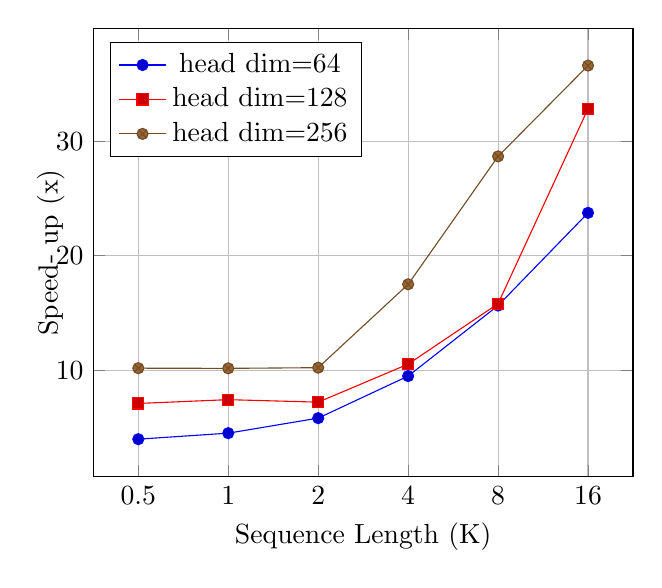
\begin{tikzpicture}
    \begin{axis}[
        title={},
        xlabel={Sequence Length (K)},
        ylabel={Speed- up (x)},
        ylabel style={yshift=-10pt},
        legend pos=north west,
        grid=both,
        xtick={512, 1024, 2048, 4096, 8192, 16384},
        xticklabels={0.5, 1, 2, 4, 8, 16},
        log ticks with fixed point,
        xmode=log,
        % ymode=log
    ]
    
    % head dim=64
    \addplot coordinates {
        (512, 10.7097 / 2.6930)
        (1024, 10.9562 / 2.4330)
        (2048, 14.0425 / 2.4151)
        (4096, 24.4682 / 2.5787)
        (8192, 47.6885 / 3.0478)
        (16384, 94.9672 / 4.0006)
    };
    \addlegendentry{head dim=64}
    
    % head dim=128
    \addplot coordinates {
        (512, 18.8856 / 2.6611)
        (1024, 19.6152 / 2.6409)
        (2048, 19.0975 / 2.6484)
        (4096, 31.2284 / 2.9655)
        (8192, 60.9088 / 3.8531)
        (16384, 191.4909 / 5.8325)
    };
    \addlegendentry{head dim=128}
    
    % head dim=256
    \addplot coordinates {
        (512, 47.2460 / 4.6427)
        (1024, 47.4189 / 4.6667)
        (2048, 47.8577 / 4.6824)
        (4096, 83.5260 / 4.7730)
        (8192, 166.8563 / 5.8201)
        (16384, 330.6606 / 9.0348)
    };
    \addlegendentry{head dim=256}
    
    \end{axis}
\end{tikzpicture}
  }
    \vspace{-1mm}
		% \caption{The x-axis is the model dimension and the y-axis is accuracy on MQAR.} 
	\caption{{Speed-up of the chunkwise parallel form vs. the recurrent form.}} 		\label{fig:kernel_speed} 
    \vspace{-5mm}
	% \end{figure}/
	\end{wrapfigure}

to rewrite most operations in matmuls. The  inverse of lower triangular matrices could be solved efficiently using forward substitution. Once computed,
the hidden state updates (Eq.~\ref{eq:delta_chunk_h}) and the output computations (Eq.~\ref{eq:delta_chunk_o}) are largely the same as in vanilla linear attention. We  adapt \textsc{FlashLinearAttention}  \cite{yang_gated_2023} to implement Eq.~\ref{eq:delta_chunk_h} and \ref{eq:delta_chunk_o} with hidden states recomputed during the backward pass for saving GPU memory. The PyTorch pseudocode for the forward pass is shown in Listing \ref{list_code}.

% and thus take $\mathcal{O}(LCd + Ld^2)$ work and $\mathcal{O}(\frac{L}{C})$ sequential steps.
% In order to save even more memory, we discard the chunk-level hidden states $\rmS_{[t]}$'s (which would take $\mathcal{O}(\frac{L}{C}d^2)$ space) after the forward pass and recompute them during the backward pass as in \citet{yang_gated_2023}.

\vspace{-2mm}
\paragraph{Speed comparison.} 
We implement both the pure recurrent form\footnote{Note that our recurrent  kernel is already 2$\times$ faster than the original CUDA kernel from \citet{schlag_linear_2021}.} and the chunkwise parallel form in Triton \cite{triton} and show the speed-ups for various sequence lengths (L) and head dimensions ($d_\text{head}$) in the right figure, where the model dimension $d$ is 2048 and we vary batch size and sequence length so that they multily to 16384.\footnote{So far we have been assuming a single head ($d_\text{head} = d$) for easier exposition. In practice we use multiple heads where the head dimension $d_\text{head}$ is smaller than the model dimension $d$. We thus have $\rmS_{t} \in \mathbb{R}^{d \times d_\text{head}}$.}
% \footnote{\url{https://github.com/IDSIA/recurrent-fwp/blob/master/algorithmic/fast_weight/fast_weight_cuda.cu}.}.
Our chunkwise algorithm achieves greater speed-ups as sequence length \( L \) and head dimension \( d_\text{head} \) increase, where the use of sequence-level parallelism (for high GPU occupancy) and tensor core (for fast matmuls) become more important \cite[][\S 3]{yang_gated_2023}. 

% \vspace{-2mm}
\paragraph{Fully Parallel Form for DeltaNet.}
For completeness, we also discuss the fully parallel form of DeltaNet. While we use the concept of a ``pseudo'' value, it is possible to avoid modifying values. From Eq.~\ref{eq:unroll}, it is straightforward to compute the attention matrix $\rmA$: $\rmA_{ij} = \vk_j^\intercal \rmP_{j+1}^i \vq_i $ if $j \le i$ and $0$ otherwise. Notably, $\rmA$ has the matrix form $
\rmA = \left(\rmQ\rmK^T \odot \rmM\right) \rmT $, obtained by combining Eq.~\ref{eq:delta_KU} and \ref{eq:wu=akv}.
However, computing $\rmT$ requires a matrix inverse (Eq.~\ref{eq:inverse}), which scales cubically with sequence length without further algorithmic changes. 
Due to the above we avoid using the fully parallel form for training DeltaNet; however the ``attention'' matrix derived from this form could be of interest to the interpretability study for RNNs \cite{ali2024hidden, DBLP:journals/corr/abs-2405-16504}.

\vspace{-2mm}
\subsection{DeltaNet Transformer}
\begin{wrapfigure}{r}{0.5\textwidth}
   \centering
   \vspace{-15mm}
   \resizebox{\linewidth}{!}{% 在定义颜色部分添加淡色版本
\definecolor{faded_oproj_color}{RGB}{239,247,241}  % 更浅的绿色
\definecolor{faded_red}{RGB}{255,235,235}          % 更浅的红色
\definecolor{faded_add_norm_color}{RGB}{250,250,230} % 更浅的黄色

% 专门为 k 分支创建新样式
\tikzset{
    stackedsmall_faded/.style={
        draw=black!20,
        very thick,
        fill=faded_oproj_color,
        minimum width=1.5cm,
        rounded corners=3pt,
        rectangle
    },
    conv_faded/.style={
        draw=black!20,
        very thick,
        minimum width=30pt,
        fill=faded_red,
        rounded corners=3pt,
        rectangle,
        font=\small
    },
    l2_faded/.style={
        draw=black!20,
        very thick,
        minimum width=30pt,
        fill=faded_add_norm_color,
        rounded corners=3pt,
        rectangle,
        font=\small
    },
    swish_faded/.style={
        draw=black!20,
        thick,
        line width=1pt,
        circle,
        minimum size=8pt,
        inner sep=0pt,
        outer sep=0pt,
        path picture={
            \draw[black!20,domain=-1.5:0, samples=50, variable=\x, thick]
            plot ({\x}, {0});
            \draw[black!20,domain=0:1.5, samples=50, variable=\x, thick]
            plot ({\x}, {\x});
        }
    }
}


\begin{tikzpicture}
    % 定义颜色
    \definecolor{fgate_color}{RGB}{252,224,225}
    \definecolor{abc_color}{RGB}{252,226,187}
    \definecolor{add_norm_color}{RGB}{242,243,193}
    \definecolor{glu_color}{RGB}{194,232,247}
    \definecolor{silu_color}{RGB}{203,231,207}
    \definecolor{linear_color}{RGB}{220,223,240}
    \definecolor{gray_bbox_color}{RGB}{243,243,244}
    \definecolor{oproj_color}{RGB}{203,231,207}
    \definecolor{operator_color}{RGB}{252,224,225}

    % 定义所有样式
    \tikzset{
        model/.style={
            draw=black,
            very thick,
            fill=gray_bbox_color,
            minimum width=4cm,
            minimum height=5.4cm,
            rounded corners=10pt
        },
        gsa/.style={
            draw=black,
            very thick,
            fill=gray_bbox_color,
            minimum width=7cm,
            minimum height=7cm,
            rounded corners=10pt
        },
        tokenmixer/.style={
            draw=black,
            very thick,
            fill=abc_color!80,
            minimum width=2.5cm,
            minimum height=0.7cm,
            rounded corners=3pt
        },
        glu/.style={
            draw=black,
            very thick,
            fill=glu_color!80,
            minimum width=2.5cm,
            minimum height=0.7cm,
            rounded corners=3pt
        },
        norm/.style={
            draw=black,
            very thick,
            fill=add_norm_color!80,
            minimum width=2.5cm,
            rounded corners=3pt,
            align=center
        },
        linear/.style={
            draw=black,
            very thick,
            fill=oproj_color!80,
            minimum width=2.5cm,
            rounded corners=3pt
        },
        stacked/.style={
            draw=black,
            very thick,
            fill=oproj_color!80,
            minimum width=2.5cm,
            rounded corners=3pt,
            rectangle
        },
        stackedsmall/.style={
            draw=black,
            very thick,
            fill=oproj_color!80,
            minimum width=1.5cm,
            rounded corners=3pt,
            rectangle
        },
        conv/.style={
            draw=black,
            very thick,
            minimum width=30pt,
            fill=red!30,
            rounded corners=3pt,
            rectangle,
            font=\small
        },
        l2/.style={
            draw=black,
            very thick,
            minimum width=30pt,
            fill=add_norm_color!80,
            rounded corners=3pt,
            rectangle,
            font=\small
        },
        fgate/.style={
            draw=black,
            very thick,
            fill=oproj_color!80,
            minimum width=1.1cm,
            rounded corners=3pt
        },
        oproj/.style={
            draw=black,
            very thick,
            fill=oproj_color!80,
            minimum width=2.5cm,
            rounded corners=3pt
        },
        silu/.style={
            draw=black,
            very thick,
            fill=silu_color,
            minimum width=1.1cm,
            rounded corners=3pt
        },
        layerlink/.style={
            -Latex,
            very thick
        },
        modulelink/.style={
            -Latex,
            very thick,
            densely dashed,
            shorten >=1pt,
            shorten <=1pt,
            rounded corners=3pt
        },
        normlink/.style={
            very thick
        },
        residual/.style={
            very thick,
            rounded corners=5pt
        },
        qf/.style={
            -Latex,
            very thick,
            rounded corners=5pt
        },
        oplus/.style={
            draw=black,
            line width=1pt,
            circle,
            minimum size=8pt,
            inner sep=0pt,
            outer sep=0pt,
            path picture={
                \draw (path picture bounding box.center) -- ++(0.3cm,0)
                (path picture bounding box.center) -- ++(-0.3cm,0)
                (path picture bounding box.center) -- ++(0,0.3cm)
                (path picture bounding box.center) -- ++(0,-0.3cm);
            }
        },
        otimes/.style={
            draw=black,
            very thick,
            circle,
            minimum size=8pt,
            inner sep=0pt,
            outer sep=0pt,
            path picture={
                \draw (path picture bounding box.center) -- ++(0.25cm,0.25cm)
                (path picture bounding box.center) -- ++(-0.25cm,-0.25cm)
                (path picture bounding box.center) -- ++(-0.25cm,0.25cm)
                (path picture bounding box.center) -- ++(0.25cm,-0.25cm);
            }
        },
        sigmoid/.style={
            draw=black,
            line width=1pt,
            circle,
            minimum size=8pt,
            inner sep=0pt,
            outer sep=0pt,
            path picture={
                \node at (path picture bounding box.center) {$\sigma$};
            }
        },
        swish/.style={
            draw=black,
            thick,
            line width=1pt,
            circle,
            minimum size=8pt,
            inner sep=0pt,
            outer sep=0pt,
            path picture={
                \draw[domain=-1.5:0, samples=50, variable=\x, blue, thick]
                plot ({\x}, {0});
                \draw[domain=0:1.5, samples=50, variable=\x, blue, thick]
                plot ({\x}, {\x});
            }
        },
        kgsa/.style={
            draw=black,
            very thick,
            fill=abc_color!50,
            minimum width=4cm,
            minimum height=0.8cm,
            rounded corners=3pt
        }
    }

    % 左侧模型结构
    \node[model] (model) at (0,0) {};
    \node[anchor=east,xshift=-2pt] at (model.west) (ntimes) {$N\times$};
    \node[below=12pt, minimum width=2.5cm] at (model.south) (input) {Inputs};
    \node[norm, anchor=south, yshift=20pt] at (model.south) (norm1) {RMSNorm};
    \draw[layerlink] (input.north) -- (norm1.south);
    \node[tokenmixer, anchor=south, yshift=8pt] at (norm1.north) (gsa0) {DeltaNet};
    \draw[normlink] (norm1.north) -- (gsa0.south);
    \node[oplus, anchor=south, yshift=4pt] at (gsa0.north) (oplus1) {};
    \node[norm, anchor=south, yshift=14pt] at (oplus1.north) (norm2) {RMSNorm};
    \draw[normlink] (gsa0.north) -- (oplus1.south);
    \draw[layerlink] (oplus1.north) -- (norm2.south);
    \draw[residual] ([yshift=-10pt]norm1.south) -- ([xshift=-48pt,yshift=-10pt]norm1.south) -- ([xshift=-48pt]oplus1.center) -- (oplus1.center);
    \node[glu, anchor=south, yshift=8pt] at (norm2.north) (glu) {SwiGLU};
    \draw[normlink] (norm2.north) -- (glu.south);
    \node[oplus, anchor=south, yshift=4pt] at (glu.north) (oplus2) {};
    \node[norm, anchor=south, yshift=10pt] at (model.north) (norm3) {RMSNorm};
    \draw[normlink] (glu.north) -- (oplus2.south);
    \draw[residual] ([xshift=0pt,yshift=8pt]oplus1.center) -- ([xshift=-48pt,yshift=8pt]oplus1.center) -- ([xshift=-48pt]oplus2.center) -- (oplus2.center);
    \node[linear, anchor=south, yshift=5pt] at (norm3.north) (linear) {Linear};
    \draw[layerlink] (oplus2.north) -- (norm3.south);
    \draw[normlink] (norm3.north) -- (linear.south);
    \node[above=12pt] at (linear.north) (output) {Outputs};
    \draw[layerlink] (linear.north) -- (output.south);

    % 右侧 - Delta Rule 实现
\node[gsa, anchor=west,xshift=25pt] (gsa) at (model.east)  {};
% \node[] at (gsa |- input) (input1) {Block Design};

\node[kgsa, yshift=15pt,minimum width=170pt] at (gsa.mid) (kernel) {Delta Rule};
\node[below=12pt] at (gsa.south) (input) {\textcolor{white}{Inputs}};

\node[stackedsmall, anchor=south, yshift=20pt] at (gsa.south) (vproj) {Linear};
\node[conv, anchor=south, yshift=8pt] at (vproj.north) (vconv) {Conv};
\node[swish, anchor=south, yshift=4pt] at (vconv.north) (vsilu) {};
\draw[layerlink] (vsilu.north) -- (vsilu|-kernel.south) node[pos=0.8, right] {$\boldsymbol{v}$};
\draw[normlink] (vsilu.south) -- (vconv.north);
\draw[normlink] (vconv.south) -- (vproj.north);
\draw[residual] (input.north) -- (gsa.south) -- (vproj.south);
% 然后使用新样式替换原来的部分
\node[stackedsmall_faded, anchor=south, yshift=19pt] at ($(gsa.south west)!0.2!(gsa.south east)$) (kproj) {Linear};
\node[conv_faded, anchor=south, yshift=8pt] at (kproj.north) (kconv) {Conv};
\node[swish_faded, anchor=south, yshift=4pt] at (kconv.north) (ksilu) {};
\node[l2_faded, anchor=south, yshift=4pt] at (ksilu.north) (kl2) {L2 Norm};
\draw[black!20, very thick] (kl2.north) -- (kl2|-kernel.south);
\draw[black!20, very thick] (ksilu.north) -- (kl2.south);
\draw[black!20, very thick] (ksilu.south) -- (kconv.north);
\draw[black!20, very thick] (kconv.south) -- (kproj.north);
\draw[black!20, very thick, rounded corners=5pt] (input.north) -- (gsa.south) |- ([xshift=-10pt,yshift=10pt]gsa.south) -| (kproj.south);


\node[stackedsmall, anchor=south, yshift=21pt] at ($(gsa.south west)!0.15!(gsa.south east)$) (qproj) {Linear};
\node[conv, anchor=south, yshift=8pt] at (qproj.north) (qconv) {Conv};
\node[swish, anchor=south, yshift=4pt] at (qconv.north) (qsilu) {};
\node[l2, anchor=south, yshift=4pt] at (qsilu.north) (ql2) {L2 Norm};
\draw[layerlink] (ql2) -- (ql2|-kernel.south) node[pos=0.5, left] {$\boldsymbol{q}$};
\draw[normlink] (qsilu.north) -- (ql2.south);
\draw[normlink] (qsilu.south) -- (qconv.north);
\draw[normlink] (qconv.south) -- (qproj.north);
\draw[residual] (input.north) -- (gsa.south) |- ([xshift=-10pt,yshift=10pt]gsa.south) -| (qproj.south);


% \node[swish, xshift=-40pt, yshift=50pt] at ($(gsa.south west)!0.375!(gsa.south east)$) (qsilu) {};
% link between qsilu and qproj
% \draw[normlink] (qsilu.south) -- (qsilu|-qproj.north);

\node[fgate, anchor=south, yshift=20pt] at ($(gsa.south west)!0.8!(gsa.south east)$)  (fproj) {Linear};
\node[sigmoid, yshift=30pt] at (fproj.north) (sigmoid) {};
\draw[qf] (sigmoid.north) -- (sigmoid.north|-kernel.south) node[pos=0.8, right] {$\boldsymbol{\beta}$};
\draw[normlink] (fproj.north) -- (sigmoid);
\draw[residual] (input.north) -- (gsa.south) |- ([xshift=10pt,yshift=10pt]gsa.south) -| (fproj.south);

% \node[stacked, anchor=south, yshift=20pt] at ($(gsa.south west)!0.88!(gsa.south east)$) (gproj) {Linear};
% \draw[residual] (input.north) -- (gsa.south) |- ([xshift=10pt,yshift=10pt]gsa.south) -| (gproj.south);
% \node[sigmoid, yshift=20pt] at (gproj.north) (sigmoid) {};
% \draw[normlink] (gproj.north) -- (sigmoid);

\node[norm, anchor=south, yshift=15pt] at (kernel.north) (norm4) {RMSNorm};
% \node[otimes, anchor=south, yshift=6pt] at (norm4.north) (otimes) {};
\node[linear, anchor=south, yshift=15pt] at (norm4.north) (oproj) {Linear};
\draw[layerlink] (kernel.north) -- (norm4.south);
\node[right] at ($(kl2)+(0,19pt)$) {$\boldsymbol{k}$};
% \draw[normlink] (norm4.north) -- (otimes.south);
\draw[normlink] (norm4.north) -- (oproj.south);
% \draw[residual] (sigmoid) |- (otimes) node[pos=0.8, above] {$\boldsymbol{g}$};

\node[above=12pt] at (gsa.north) (output) {\textcolor{white}{Outputs}};
\draw[layerlink] (oproj.north) -- (output.south);
    % \draw[modulelink] (gsa0.east) -- (kernel.west);
    \draw[modulelink] (gsa0.east) -- ++(12pt,0) |- (kernel.west);
\end{tikzpicture}
}
   \vspace{-8mm}
   \caption{An illustration of DeltaNet neural architecture.}
   \label{fig:enter-label}
   \vspace{-10mm}
\end{wrapfigure}

We describe how the DeltaNet layer primitive is used to build up a transformer-like model using standard modules. We largely  follow the LLaMA-architecture  \cite[Transformer++,][]{touvron2023llama} and simply replace the self-attention layer with the DeltaNet layer. We also apply normalization before output projection for stable training \cite{qin_devil_2022, Mercat2024LinearizingLL}. As the additional parameters for computing scalar $\beta_t$ terms are negligible,  parameter allocation is roughly the same as in Transformer++, i.e., $4d^2$ for the DeltaNet layer  and $8d^2$ for the SwiGLU FFN layer \cite{shazeer2020glu}. 
\vspace{-2mm}
\paragraph{Feature map and normalization.} 
Our key/query vectors are given by $\vk_t = \frac{\text{SiLU}(\rmW_{K}\vx_t)}{\Vert \text{SiLU}(\rmW_{K}\vx_t)\Vert_2}$, $\vq_t = \frac{\text{SiLU}(\rmW_{Q}\vx_t)}{\Vert \text{SiLU}(\rmW_{Q}\vx_t)\Vert_2}$.  \citet{schlag_linear_2021} originally follow \citet{katharopoulos_transformers_2020} and apply a ``$\text{ELU}+1$'' \cite{clevert_fast_2016} to nonlineary transform the key/query vectors. We instead use the $\text{SiLU}$ activation \cite{elfwing_sigmoid-weighted_2017}, which was found to perform better \cite{qin2023scaling, mamba2}.
For stability, it is crucial to ensure that the norm of each eigenvalue of the transition matrices does not exceed one.  The eigenvalues of $\rmI - \beta_t \vk_t \vk_t^\intercal$ are 1 with multiplicity \(d-1\) and \(1 - \beta_t \|\vk_t\|_2\) with multiplicity 1. \citet{schlag_linear_2021} used the $L_1$ norm to normalize query/key vectors, ensuring that $
0 \leq 1 - \beta_t \| \vk_t\|_2 \leq 1$. We instead apply $L_2$ normalization, which we found to perform better and offers a more intuitive interpretation: when $\beta_t=1$, $\rmI-\vk_t \vk_t^\intercal$ becomes a projection matrix, erasing information in one subspace while preserving the other $d-1$ subspaces. This is beneficial for retaining information while enabling more \emph{targeted} forgetting. 
% This also gives us a more intuitive understanding of delta rule: if $\$ we have a set of keys $[k1, \cdots k_n]$. For each time step $t$, each key $k_i$ will erase its components 


\vspace{-2mm}
 \subsection{Hybrid Models}
 \vspace{-2mm}
Following recent work on combining subquadratic token-mixing layers with existing neural network primitives \citep{arora_simple_2024,de_griffin_2024,Lieber2024JambaAH}, we also experiment with hybridizing DeltaNet models.

 \vspace{-2mm}
\paragraph{Convolutional layers.} Recent linear recurrent models typically incorporate a lightweight depthwise-separable convolution layer after the query/key/value projections \cite{gu_mamba_2023,beck2024xlstm,mamba2}. This ``short convolution'' layer \cite{poli_hyena_2023} generalizes the shift SSM \cite{fu_hungry_2023}, and is
 efficient in both number of parameters  and computational cost. We also add a short convolution layer after the query/key/value projections. 
 
 % Empirically, we found short convolutions to be crucial for DeltaNet performance on real-world tasks, and for Mamba on synthetic in-context learning tasks. 

\vspace{-2mm}
\paragraph{Local sliding window and global attention.}
 Linear attention largely uses a content-based addressing mechanism \cite{graves_neural_2014} and lacks positional information \cite{zhang_linear_2023}. \citet{arora_simple_2024} also argue that linear attention lacks the ability to perform precise local token shifts and comparisons, thus facing difficulties on  retrieval-intensive tasks.   
  Motivated by this, we experiment with two different hybrid architectures that incorporate softmax attention. We first explore \textit{ sliding window attention} (SWA) which has been shown to significantly improve linear attention \cite{qin_devil_2022, arora_simple_2024, lingle_transformer-vq_2023, nahshan_linear_2024}; we follow Griffin \cite{de_griffin_2024} and Samba \cite{ren2024samba}  to interleave DeltaNet layers and SWA layers. We also experiment with \textit{global attention}, which has been found to be helpful  \cite{lei_when_2021, huang_encoding_2022} even if only few of the recurrent layers are replaced with global attention \cite{Lieber2024JambaAH}. We follow \citet{fu_hungry_2023} to replace only two layers with global attention: the second layer and the $(\frac{N}{2}+1)$-th  layer, where $N$ is total number of layers.
